%!TEX root = ../main.tex

\begin{figure}[ht]
  \centering
  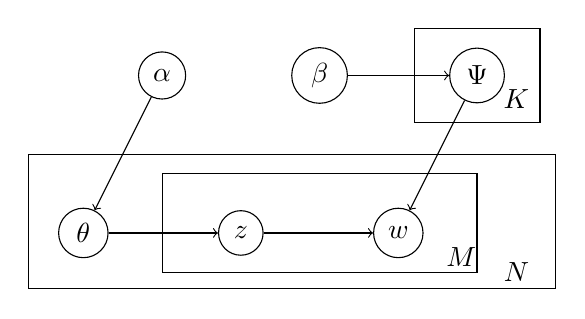
\begin{tikzpicture}
    \node (theta) at (0,0) [circle, draw] {$\theta$};
    \node (z) at (2,0) [circle, draw] {$z$};
    \node (w) at (4,0) [circle, draw] {$w$};
    \node (alpha) at (1,2) [circle, draw] {$\alpha$};
    \node (psis) at (5,2) [circle, draw] {$\Psi$};
    \node (b) at (3,2) [circle, draw] {$\beta$};

    \draw[->] (alpha) -- (theta);
    \draw[->] (b.east) -- (psis.west);

    \draw[->] (theta.east) -- (z.west);
    \draw[->] (z.east) -- (w.west);
    \draw[->] (psis) -- (w);

    \draw (-.7,-.7) rectangle (6.,1);
    \draw (1,-.5) rectangle (5,.75);
    \draw (4.2,1.4) rectangle (5.8,2.6);

    \node at (5.5,-.5) {$N$};
    \node at (4.8,-.3) {$M$};
    \node at (5.5,1.7) {$K$};
  \end{tikzpicture}

  \caption{Model}
  \label{fig:chapter3-model}
\end{figure}

\section{Population and Methods}

\subsection{Determine companies, keywords and stock symbols to analyze}

First, a list of automotive companies is needed.
These companies must be traded on a stock exchange to perform the comparison with tweet sentiments.
As a single company may own several car brands a list of all brands has been set up.
The result of the analysis is depicted in \autoref{tab:brands}.
Both brands which aren't customer facing passenger car brands and brands which do not longer exist have been omitted.
Furthermore, the brands have been grouped by their owning company.

  \begin{longtable}[c]{ll}
   \bfseries{Car brand} & \bfseries{Owning Company}  \\ \hline
  \endfirsthead
  %
  \multicolumn{2}{c}%
  {{\bfseries Table \thetable\ continued from previous page}} \\
   &  \\
  \endhead
  %
  BMW  & BMW \cite[p.30]{BMWGroup2017} \\
  Mini  & BMW  \cite[p.30]{BMWGroup2017} \\
  Rolls-Royce   & BMW \cite[p.30]{BMWGroup2017} \\
  Mercedes-AMG & Daimler \cite[p.90]{DaimlerAG2018} \\
  Mercedes-Benz  & Daimler \cite[p.90]{DaimlerAG2018} \\
  Mercedes-Maybach & Daimler \cite[p.90]{DaimlerAG2018} \\
  Smart  & Daimler \cite[p.90]{DaimlerAG2018} \\
  Alfa Romeo & Fiat Chrysler Automobiles \cite[p.32]{FiatChryslerAutomobiles2018a} \\
  Chrysler & Fiat Chrysler Automobiles \cite[p.32]{FiatChryslerAutomobiles2018a} \\
  Dodge & Fiat Chrysler Automobiles \cite[p.32]{FiatChryslerAutomobiles2018a} \\
  Fiat & Fiat Chrysler Automobiles \cite[p.32]{FiatChryslerAutomobiles2018a} \\
  Fiat Professional & Fiat Chrysler Automobiles \cite[p.32]{FiatChryslerAutomobiles2018a} \\
  Jeep & Fiat Chrysler Automobiles \cite[p.32]{FiatChryslerAutomobiles2018a} \\
  Lancia & Fiat Chrysler Automobiles \cite[p.32]{FiatChryslerAutomobiles2018a} \\
  RAM & Fiat Chrysler Automobiles \cite[p.32]{FiatChryslerAutomobiles2018a} \\
  Ford & Ford Motor Company \cite[p.18]{FordMotorCompany2018} \\
  Lincoln  & Ford Motor Company \cite[p.18]{FordMotorCompany2018} \\
  Baojun & General Motors Company \cite[p.1]{GeneralMotorsCompany2018} \\
  Buick & General Motors Company \cite[p.1]{GeneralMotorsCompany2018} \\
  Cadillac & General Motors Company \cite[p.1]{GeneralMotorsCompany2018} \\
  Chevrolet & General Motors Company \cite[p.1]{GeneralMotorsCompany2018} \\
  GMC & General Motors Company \cite[p.1]{GeneralMotorsCompany2018} \\
  Holden & General Motors Company \cite[p.1]{GeneralMotorsCompany2018} \\
  Jiefang & General Motors Company \cite[p.1]{GeneralMotorsCompany2018} \\
  Wuling & General Motors Company \cite[p.1]{GeneralMotorsCompany2018} \\
  Honda & Honda \cite[p.3]{HondaMotorCo.2017} \\
  Hyundai & Hyundai Motor Company \cite[p.127]{HyundaiMotorCompany2016} \\
  KIA & Hyundai Motor Company \cite[p.127]{HyundaiMotorCompany2016} \\
  Datsun & Nissan Motor Corporation \cite[p.5]{NissanMotorCorporation2017} \\
  Infinity & Nissan Motor Corporation \cite[p.5]{NissanMotorCorporation2017} \\
  Nissan & Nissan Motor Corporation \cite[p.5]{NissanMotorCorporation2017} \\
  Citroën & Groupe PSA \cite[p.3]{GroupePSA2018} \\
  Opel & Groupe PSA \cite[p.3]{GroupePSA2018} \\
  Peugeot& Groupe PSA \cite[p.3]{GroupePSA2018} \\
  Vauxhall & Groupe PSA \cite[p.3]{GroupePSA2018} \\
  Alpine & Groupe Renault \cite[p.11]{GroupeRenault2018} \\
  Dacia & Groupe Renault \cite[p.11]{GroupeRenault2018} \\
  Lada & Groupe Renault \cite[p.11]{GroupeRenault2018} \\
  Renault & Groupe Renault \cite[p.10]{GroupeRenault2018} \\
  Renault Samsung Motors & Groupe Renault \cite[p.10]{GroupeRenault2018} \\
  Daihatsu & Toyota Motor Corporation \cite[p.2]{ToyotaMotorCorporation2018} \\
  Lexus & Toyota Motor Corporation \cite[p.2]{ToyotaMotorCorporation2018} \\
  Toyota & Toyota Motor Corporation \cite[p.2]{ToyotaMotorCorporation2018} \\
  Audi & Volkswagen AG \cite[p.104]{VolkswagenAktiengesellschaft2017} \\
  Bentley & Volkswagen AG \cite[p.104]{VolkswagenAktiengesellschaft2017} \\
  Bugatti & Volkswagen AG \cite[p.104]{VolkswagenAktiengesellschaft2017} \\
  Lamborghini & Volkswagen AG \cite[p.104]{VolkswagenAktiengesellschaft2017} \\
  Porsche & Volkswagen AG \cite[p.104]{VolkswagenAktiengesellschaft2017} \\
  Seat & Volkswagen AG \cite[p.104]{VolkswagenAktiengesellschaft2017} \\
  Škoda & Volkswagen AG \cite[p.104]{VolkswagenAktiengesellschaft2017} \\
  Volkswagen & Volkswagen AG \cite[p.104]{VolkswagenAktiengesellschaft2017} \\ \hline
  
  \caption{Automotive brands and their corresponding owning company}
  \label{tab:brands}
  \end{longtable}

According to the survey of \emph{World Motor Vehicle Production 2016} the biggest five car manufacturing companies are: Toyota, Volkswagen, Hyundai, General Motors and Ford \cite{OICA2016}.
Therefore the study will focus on these five companies.
The count of manufactured cars and the companies stock symbol are summarized in \autoref{tab:companies-counts-and-symbols}.
The containing symbols in the table are derived by using Yahoo Finance portal (\url{https://finance.yahoo.com}).

\begin{table}
	\begin{tabular}[c]{lrll}
	  \textbf{Company} & \textbf{\#cars \cite{OICA2016}} & \textbf{Stock Exchange} & \textbf{Symbol}  \\ \hline
	   %s
	  Ford Motor Company & 6,429,485 & New York \cite{FordMotorCompany2018} & F  \\
	  General Motors Company & 7,793,066 & New York \cite[p.17]{GeneralMotorsCompany2018} & GM \\
	  Hyundai Motor Company & 7,889,538 & Korea \cite[p.92]{HyundaiMotorCompany2016} & 005380.KS \\
	  Toyota Motor Corporation & 10,213,486 & Tokyo \cite{ToyotaMotorCorporation2018} & 7203.T \\
	  Volkswagen AG & 10,126,281 & Frankfurt \cite[p.110]{VolkswagenAktiengesellschaft2017} & VOW.F \\  \hline
	\end{tabular}
	\caption{Automotive companies and their corresponding produced cars and stock symbol}
	\label{tab:companies-counts-and-symbols}
\end{table}

\subsection{Gather tweets and stock prices}

Tweets have been captured between February 28th 2018 till September 6th 2018.
The number of collected tweets can be seen in \autoref{tab:companies-numberoftweets}.

\begin{table}
  \centering
  \begin{tabular}[h]{l r}
  \textbf{Company} & \textbf{\# of tweets} \\ \hline
    Ford & 4518198 \\
    General Motor & 575547 \\
    Hyundai & 1895306 \\
    Toyota & 915868 \\
    Volkswagen & 8244083 \\ \hline
    Total & 16149002 \\ \hline
  \end{tabular}

  \caption{Numbers of collected tweets}
  \label{tab:companies-numberoftweets}
\end{table}

The stock data can be downloaded at any point of time for the given research period and a daily frequency using the Yahoo Finance API.

% \subsection{Normalization of tweets}
% \subsection{Determine sentiment of tweets}
% \subsection{Comparing sentiment time series with share prices}